\documentclass{article}
\usepackage{bm}
\usepackage{amsmath}
\usepackage{graphicx}
\usepackage{mdwlist}
\usepackage[colorlinks=true]{hyperref}
\usepackage{geometry}
\usepackage{kotex}
\geometry{margin=1in}
\geometry{headheight=2in}
\geometry{top=2in}
\usepackage{palatino}
%\renewcommand{\rmdefault}{palatino}
\usepackage{fancyhdr}
\usepackage{indentfirst}

\newcommand{\red}[1]{{\color{red} #1}}
\newcommand{\blue}[1]{{\color{blue} #1}}
\newcommand{\orange}[1]{{\color{orange} #1}}
\newcommand{\purple}[1]{{\color{purple} #1}}

%\pagestyle{fancy}
\rhead{}
\lhead{}
\chead{%
  {\vbox{%
      \vspace{2mm}
      \large
      Statistics Lab 033.020\hfill
\\
      Seoul National University
      \\[4mm]
      \textbf{Assignment \#2} \\
      \texttt{2016-19516, Sangjun Son}
    }
  }
}

%%%%%%%%%%%%%%%%%%%%%%%
\usepackage{xcolor}
\usepackage{listings}
\definecolor{vgreen}{RGB}{104,180,104}
\definecolor{vblue}{RGB}{49,49,255}
\definecolor{vorange}{RGB}{255,143,102}

\lstdefinestyle{r-style}
{
    language=R,
    basicstyle=\scriptsize\ttfamily,
    keywordstyle=\color{vblue},
    identifierstyle=\color{black},
    commentstyle=\color{vgreen},
    numbers=left,
    numberstyle=\tiny\color{black},
    numbersep=10pt,
    tabsize=8,
    moredelim=*[s][\colorIndex]{[}{]},
    literate=*{:}{:}1
}

\lstdefinestyle{out-style}
{
    language=R,
    basicstyle=\scriptsize\ttfamily,
    numbersep=10pt,
    tabsize=8,
    moredelim=*[s][\colorIndex]{[}{]},
    literate=*{:}{:}1
}

\makeatletter
\newcommand*\@lbracket{[}
\newcommand*\@rbracket{]}
\newcommand*\@colon{:}
\newcommand*\colorIndex{%
    \edef\@temp{\the\lst@token}%
    \ifx\@temp\@lbracket \color{black}%
    \else\ifx\@temp\@rbracket \color{black}%
    \else\ifx\@temp\@colon \color{black}%
    \else \color{vorange}%
    \fi\fi\fi
}
\makeatother

\usepackage{trace}
%%%%%%%%%%%%%%%%%%%%%%%

\usepackage{paralist}

\usepackage{todonotes}
\setlength{\marginparwidth}{2.15cm}

\usepackage{tikz}
\usetikzlibrary{positioning,shapes,backgrounds}

\begin{document}

\pagestyle{fancy}

\section*{Example 1 $\sim$ 6}
(\textbf{Example 1}) \texttt{genhlth} 변수에 대해 적절한 방법을 이용하여 요약해보자. 범주형 자료의 경우에는 어떠한 요약 방법을 사용할 수 있는가?
\begin{lstlisting}[style={r-style}]
cdc <- read.table("cdc.txt", header=T)
table(cdc$genhlth)
\end{lstlisting}
\begin{lstlisting}[style={out-style}]
excellent      fair      good      poor very good 
     4657      2019      5675       677      6972 
\end{lstlisting}
\emph{Explanation: 범주형 자료의 요약은 분할표를 이용할 수 있다. 분할표를 작성하는 기본 함수는 table()을 사용한다. 전반적인 건강상태를 나타내는 genhlth의 범주별로 도수 분포표를 작성한다.} \\

(\textbf{Example 2}) \texttt{weight} 변수에 대한 수치적 요약 값을 구해보자. 전체 응답자의 평균 몸무게는 얼마인가?
\begin{lstlisting}[style={r-style}]
summary(cdc$weight)
\end{lstlisting}
\begin{lstlisting}[style={out-style}]
   Min. 1st Qu.  Median    Mean 3rd Qu.    Max. 
   68.0   140.0   165.0   169.7   190.0   500.0 
\end{lstlisting}
\emph{Explanation: 숫자형 자료의 요약은 데이터를 '최소값, 제 1사분위수, 중앙값, 제 3사분위수, 최대값'으로 요약한다. 다섯 수치 요약인 fivenum(x) 또는 이들에 평균을 포함한 summary(x)를 통해 계산해준다. 체중 (pound)에 대한 대표값이며 전체 응답자의 평균 몸무게 (Mean)은 169.7 lb $\approx$ 76.97 kg 이다.} \\

(\textbf{Example 3}) \texttt{weight} 변수와 \texttt{wtdesire} 변수의 산점도를 그려보자. 두 변수 사이에는 어떠한 관계가 
존재한다고 보여지는가? 두 변수의 상관계수는 무엇은 나타내고 있는가?
\begin{lstlisting}[style={r-style}]
plot(cdc$weight, cdc$wtdesire, 
     main="Weight & Desired weight (lb)")
cor(cdc$weight, cdc$wtdesire)
\end{lstlisting}
\begin{figure}[htb!]
    \centering
    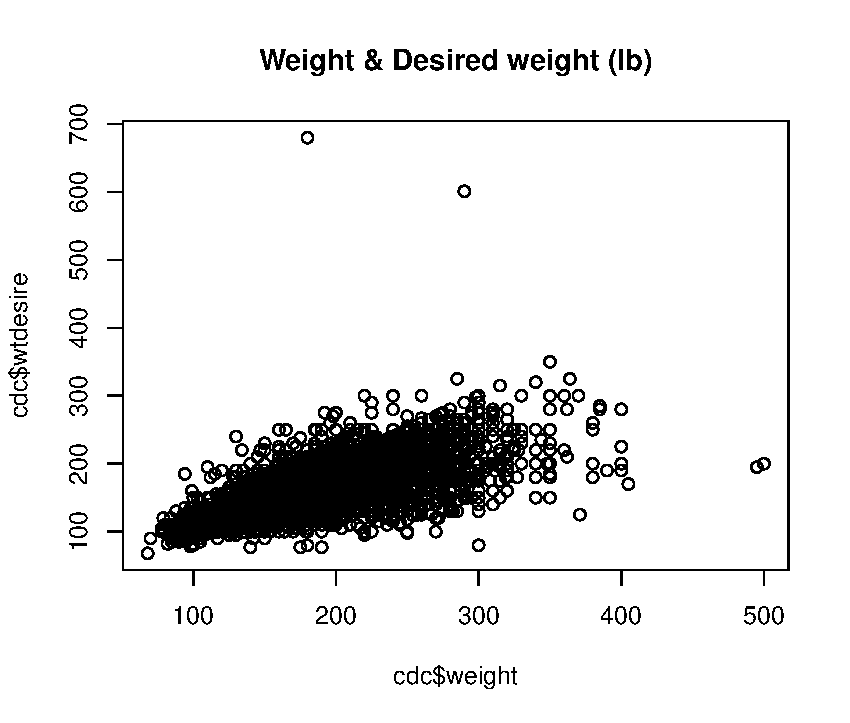
\includegraphics[width=0.5\textwidth]{fig/ex3.pdf}
    \label{fig:ex3}
\end{figure}
\begin{lstlisting}[style={out-style}]
[1] 0.8000521
\end{lstlisting}
\emph{Explanation: 그래프를 이용한 이변량 자료의 요약은 산점도(scatter plot)를 이용할 수 있다. 산점도를 그리기 위해서는 plot() 함수를 사용할 수 있다. 몸무게가 많이 나갈 수록 원하는 체중 값도 선형적으로 비례하는 것을 눈으로 확인할 수 있다. 이를 상관계수 $\rho = 0.8000521 \approx 1.0$ 임을 통해 두 변수 weight와 wtdesire 변수가 서로 선형적 관계를 가짐을 알 수 있다.} \\

(\textbf{Example 4}) \texttt{wtdesire} 변수와 \texttt{weight} 변수의 차를 계산하여 새로운 변수 \texttt{wdiff} 를 만들어보자. \texttt{wdiff} 의 분포는 어떠한가? 수치적 요약과 그래프 요약을 통해 살펴보자. 이것이 의미하는 바는 무엇인가?
\begin{lstlisting}[style={r-style}]
wdiff <- cdc$wtdesire - cdc$weight
summary(wdiff)
plot(wdiff,    main="Desired weight change (lb)")
boxplot(wdiff, main="Desired weight change (lb)")
\end{lstlisting}
\begin{lstlisting}[style={out-style}]
   Min. 1st Qu.  Median    Mean 3rd Qu.    Max. 
-300.00  -21.00  -10.00  -14.59    0.00  500.00 
\end{lstlisting}
\begin{figure}[htb!]
    \centering
    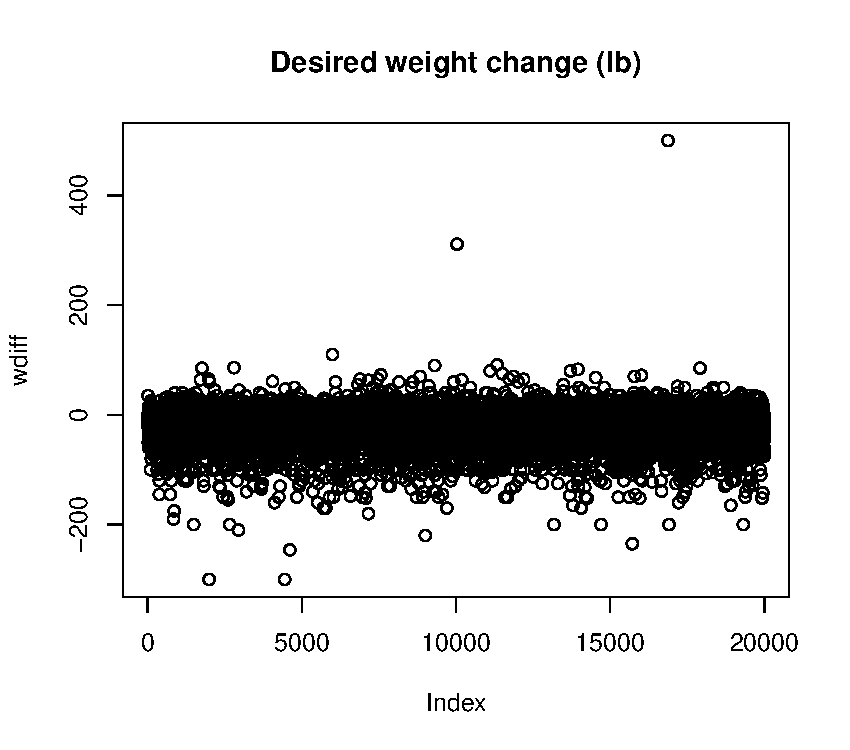
\includegraphics[width=0.5\textwidth]{fig/ex4.pdf}
    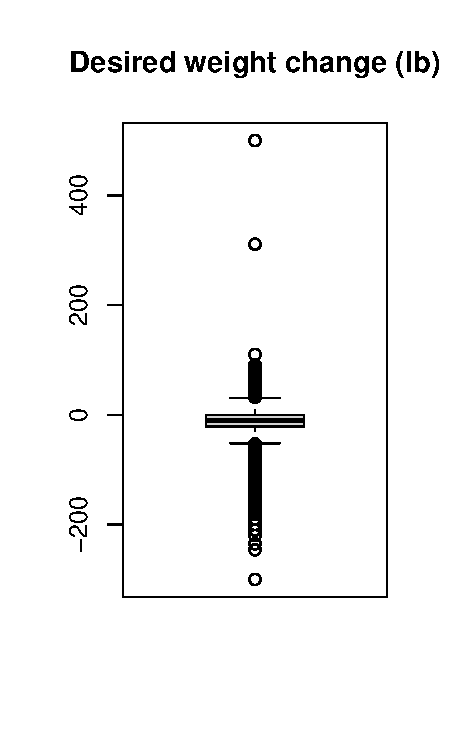
\includegraphics[width=0.25\textwidth]{fig/ex4-1.pdf}
    \label{fig:ex4}
\end{figure}
\emph{Explanation: wtdesire와 weight를 원소별 차이를 구한 변수를 wdiff로 저장하고 요약한 결과이다. outlier가 있지만 수치요약 summary()를 통해 분위수를 확인하면 대부분 음수의 값을 가지는 것을 확인 가능하다. 인덱스별로 그리는 함수 plot()와 상자그림 boxplot()을 통해 전체 응답자들이 평균적으로 체중감량을 원하는 것을 확인할 수 있다. }  \\

\newpage
(\textbf{Example 5}) \texttt{age} 변수를 이용하여 히스토그램을 그려보자. 그리고 구간의 수를 50, 100으로 바꿔가며 동일한 히스토그램을 그린 후 비교해보자.
\begin{lstlisting}[style={r-style}]
hist(cdc$age, breaks=50,  main="Age Hist w. 50 breaks")
hist(cdc$age, breaks=100, main="Age Hist w. 100 breaks")
\end{lstlisting}
\begin{figure}[htb!]
    \centering
    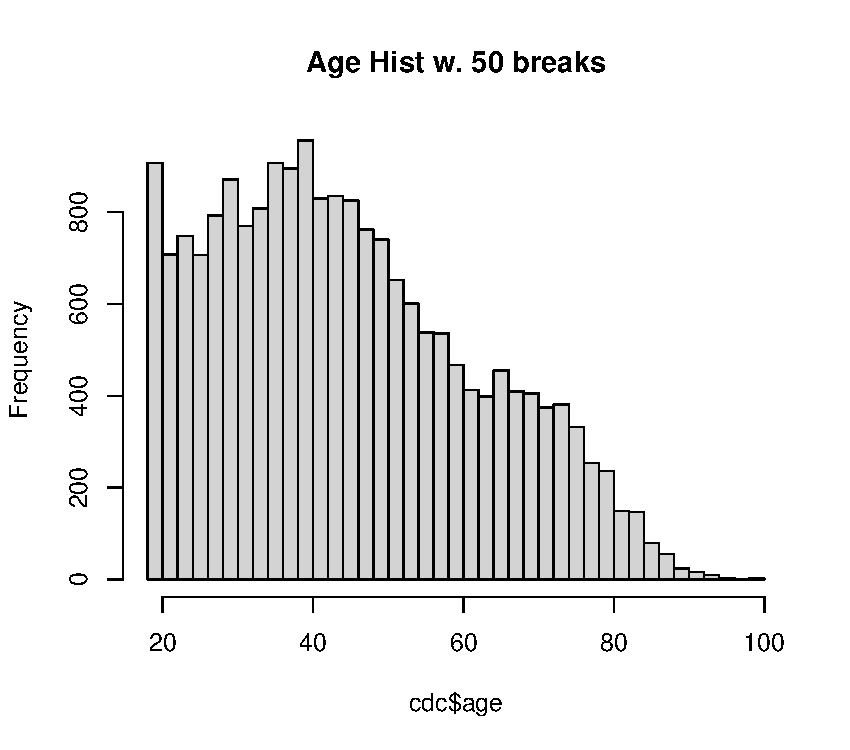
\includegraphics[width=0.4\textwidth]{fig/ex5-0.pdf}
    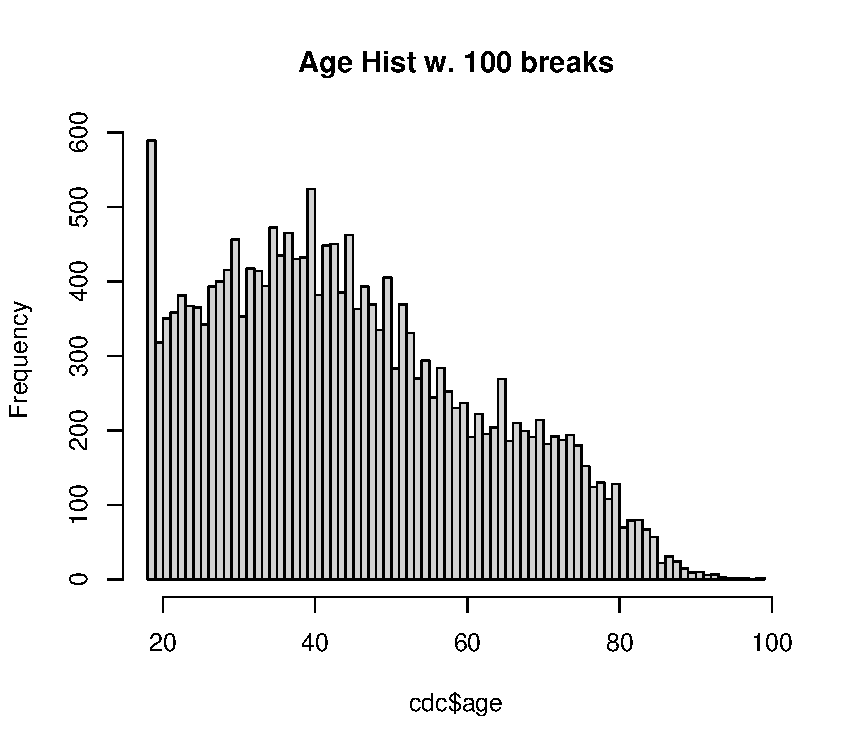
\includegraphics[width=0.4\textwidth]{fig/ex5-1.pdf}
    \label{fig:ex5}
\end{figure}
\emph{Explanation: 일변량 자료의 분포를 알아보는데 유용한 그래프는 히스토그램 hist()이다.히스토그램의 모양을 결정짓는 요소들 중 한 가지는 막대의 너비, 즉 각 막대가 나타내는 구간이다. 구간의 수를 의미하는 breaks를 달리하며 히스토그램을 다르게 표현 가능하다. 구간을 많이 할 수록 분포의 모양을 자세히 파악할 수 있다.} \\

(\textbf{Example 6}) \texttt{height} 변수와 \texttt{weight} 변수의 산점도를 그리고, 그래프의 제목은 correlation of height and weight로, x축의 이름은 \texttt{height}, y축의 이름은 \texttt{weight} 로 붙여보자.
\begin{lstlisting}[style={r-style}]
plot(cdc$height, cdc$weight, 
     main="correlation of height and weight",
     xlab="height", ylab="weight")
cor(cdc$height, cdc$weight)
\end{lstlisting}
\begin{figure}[htb!]
    \centering
    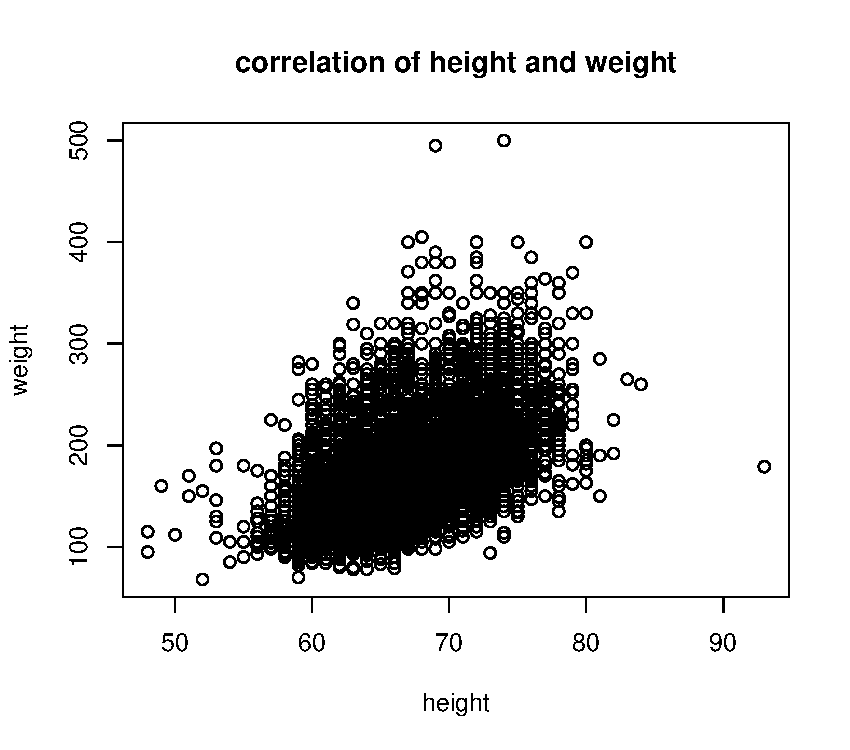
\includegraphics[width=0.45\textwidth]{fig/ex6.pdf}
    \label{fig:ex6}
\end{figure}
\begin{lstlisting}[style={out-style}]
[1] 0.5553222
\end{lstlisting}
\emph{Explanation: plot() 함수에는 다양한 하위레벨 선택사항들이 있는데 이를 사용하여 다양한 형태의 그래프를 그릴 수 있다. main 파라미터를 통해 제목을 xlab과 ylab을 통해 x, y 축명을 지정할 수 있다.} \\

\section*{Example 7 $\sim$ 9}

(\textbf{Example 7}) 범주형 자료인 \texttt{sex} 변수를 적절한 방법으로 요약해보고 이를 통해 여성과 남성의 수를 구하라.
\begin{lstlisting}[style={r-style}]
bodydims <- read.csv("bodydims.csv", header=T)
table(bodydims$sex)
\end{lstlisting}
\begin{lstlisting}[style={out-style}]
  0   1 
260 247 
\end{lstlisting}
\emph{Explanation: 범주형 자료이므로 분햘 표를 이용해 응답자의 성별 (1: 남성, 0: 여성)을 나타내는 sex의 범주별로 도수 분포표를 작성한다. 남성은 247명, 여성은 260명, 합이 507명임을 확인하였다.} \\

(\textbf{Example 8}) 전체 응답자의 양쪽 팔꿈치 지름의 합의 평균, 표준편차, 사분위값, 합, 범위(range)를 구하여라.
\begin{lstlisting}[style={r-style}]
summary(bodydims$elb.di)
\end{lstlisting}
\begin{lstlisting}[style={out-style}]
   Min. 1st Qu.  Median    Mean 3rd Qu.    Max. 
   9.90   12.40   13.30   13.39   14.40   16.70
\end{lstlisting}
\emph{Explanation: 양쪽 팔꿈치 지름을 나타내는 변수 elb.di는 숫자형 자료의 요약이므로 데이터를 '최소값, 제 1사분위수, 평균, 중앙값, 제 3사분위수, 최대값'으로 요약한다. } \\

(\textbf{Example 9}) 남성과 여성의 신장에 대해 각각 히스토그램을 그려보고, 분포를 비교하라.
\begin{lstlisting}[style={r-style}]
male   = bodydims[bodydims$sex == 1, ]
female = bodydims[bodydims$sex == 0, ]

hist(male$hgt, ylim=c(0,100), xlim=c(140,200), main="height of males")
hist(female$hgt, ylim=c(0,100), xlim=c(140,200), main="height of females")
\end{lstlisting}
\begin{figure}[htb!]
    \centering
    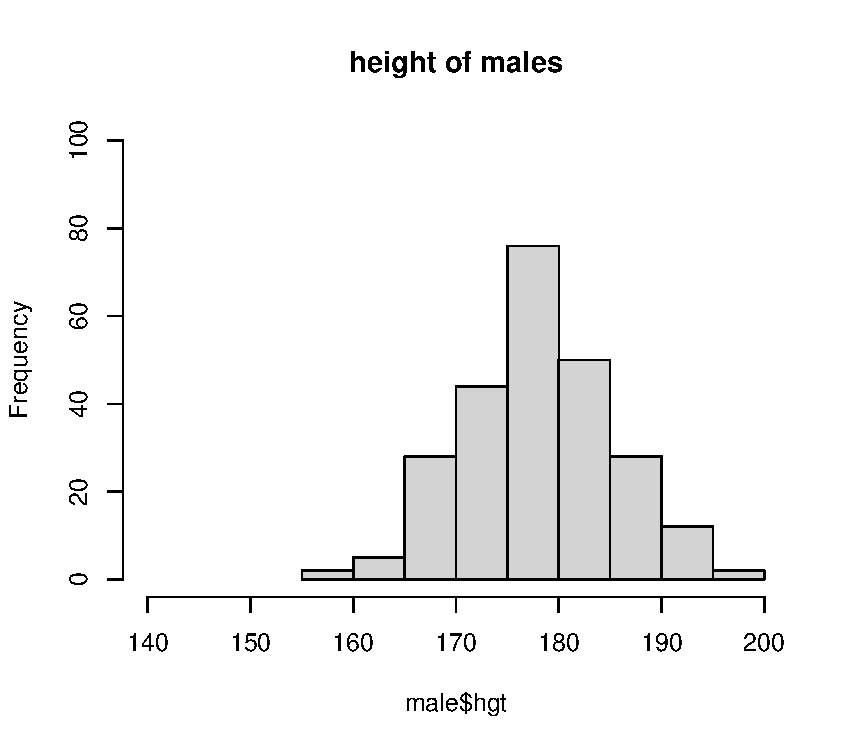
\includegraphics[width=0.49\textwidth]{fig/ex9-0.pdf}
    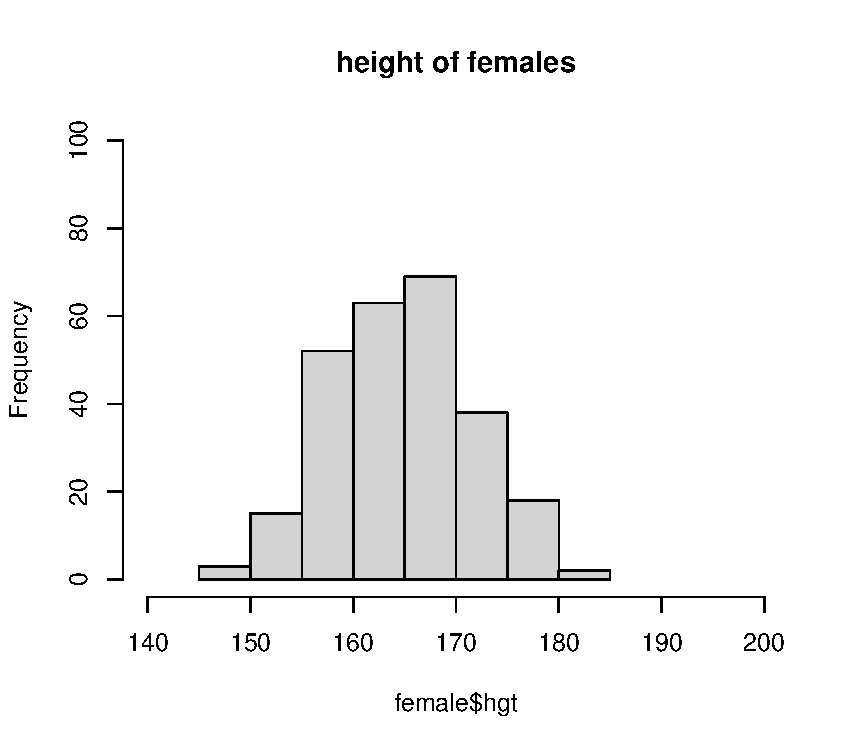
\includegraphics[width=0.49\textwidth]{fig/ex9-1.pdf}
    \label{fig:ex9}
\end{figure}
\emph{Explanation: 전체 응답자의 자료를 성별로 나누기 위해 filtering을 하기 위해 인덱스 부분에 조건을 입력하여 남성/여성을 구분하여 각각의 변수 male과 female에 대입하였다. 이에 대한 히스토그램을 같은 x축, y축 범위로 설정하여 그렸다. 남성의 신장의 분포의 중심이 여성보다 오른쪽에 있는 것으로 보아 대체적으로 더 큰 신장을 가지는 것을 확인할 수 있다.} \\

\end{document}
